\subsection{Double beta decay modes} \label{subsec:bbmodes}
%
Double beta decay is a rare nuclear transition in which a nucleus with $Z$ protons decays into a nucleus with $Z+2$ protons and the same mass number $A$. The decay can occur only if the initial nucleus is less bound than the final nucleus, and both more than the intermediate one, as shown in Fig.~\ref{fig:atomicmasses_a136}. Such a condition is fulfilled by 35 nuclides in nature because of the nuclear pairing force (see Sect.~\ref{subsec:manybody}), ensuring that nuclei with even $Z$ and $N$ are more bound than the odd-odd nuclei with the same $A=Z+N$.

\begin{figure}[tb]
\centering
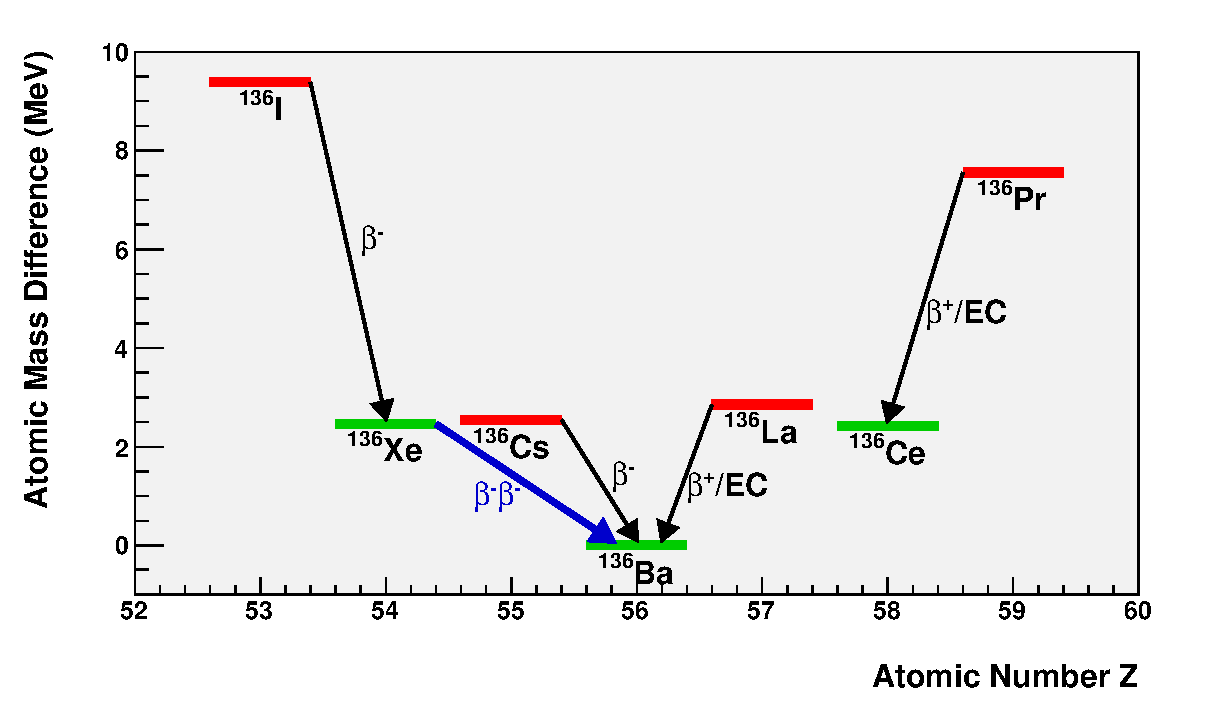
\includegraphics[width=\textwidth]{img/atomicmasses_a136.eps}
\caption{Atomic masses of isotopes with $A=136$ given as differences with respect to the most bound isotope, $^{136}\text{Ba}$. The red (green) levels indicate odd-odd (even-even) nuclei. The arrows $\beta^-$, $\beta^+$, $\beta^-\beta^-$ indicate nuclear decays accompanied by electron, positron and double electron emission, respectively. The arrows EC indicate electron capture transitions.} \label{fig:atomicmasses_a136}
\end{figure}

The standard decay mode (\bbtnu), consisting of two simultaneous beta decays,
\begin{equation}
(Z,A) \rightarrow (Z+2,A) + 2\ e^{-} + 2\ \overline{\nu}_{e},
\label{eq:bb2nu}
\end{equation}
was first considered by Maria Goeppert-Mayer in 1935 \cite{Goeppert-Mayer:1935uil}. Total lepton number is conserved in this mode, and the process is allowed in the Standard Model of particle physics. This process was first detected in 1950 using geochemical techniques \cite{Inghram:1950qv}. The first direct observation of \bbtnu\ events, in \Se{82} and using a time projection chamber, did not happen until 1987 \cite{Elliott:1987kp,Moe:2014ioa}. Since then, it has been repeatedly observed in several nuclides. Typical lifetimes are of the order of $10^{19}$--$10^{21}$ years, among the longest ever observed among radioactive decay processes\footnote{To our knowledge, only the closely related two-neutrino double electron capture process of \Xe{124}, with a half-life of $(1.8\times 0.5)\times 10^{22}$~yr \cite{XENON:2019dti}, has been measured directly to have a longer half-life than the \bbtnu\ processes in Table~\ref{tab:bb2nu_exp}.}. For a list of \bbtnu\ half-lives measured in several isotopes, see Table~\ref{tab:bb2nu_exp} \cite{Barabash:2020nck}. The longest half-life in Table~\ref{tab:bb2nu_exp} is the one for \Xe{136}, which was measured for the first time only in 2011 \cite{EXO-200:2011xzf}.

%%%%%
\begin{table}[tb]
\caption{Current best direct measurements of the half-life of \bbtnu\ processes.  The values reported are taken from the averaging procedure described in \cite{Barabash:2020nck}.} \label{tab:bb2nu_exp}
\begin{center}
%\begin{tabular}{rcc}
\begin{tabular}{p{0.10\textwidth}p{0.22\textwidth}p{0.55\textwidth}}
\toprule
Isotope & $T_{1/2}^{2\nu}\ \text{(year)}$ & Experiments \\ \midrule
%
\Ca{48} & $(5.3^{+1.2}_{-0.8}) \times 10^{19}$ & Irvine TPC \cite{Balysh:1996vr}, TGV \cite{Brudanin:2000in}, NEMO-3 \cite{NEMO-3:2016mvr}  \\
%
\Ge{76} & $(1.88\pm 0.08)\times 10^{21}$ & HEIDELBERG-MOSCOW \cite{Dorr:2003gf}, GERDA \cite{Agostini:2015nwa}  \\
%
\Se{82} & $(0.87\pm ^{+0.02}_{-0.01})\times 10^{20}$ & NEMO-3 \cite{Arnold:2018tmo}, CUPID-0 \cite{Azzolini:2019yib}, Irvine TPC \cite{Elliott:1992cf}, NEMO-2 \cite{NEMO:1997rel}   \\
%
\Zr{96} & $(2.3\pm 0.2)\times 10^{19}$ & NEMO-2 \cite{Arnold:1999vg}, NEMO-3 \cite{NEMO-3:2009fxe} \\
%
\Mo{100} & $(7.06^{+0.15}_{-0.13})\times 10^{18}$ & NEMO-3 \cite{NEMO-3:2019gwo}, CUPID-Mo \cite{Armengaud:2019rll}, NEMO-2 \cite{NEMO:1994sst}, Irvine TPC \cite{DeSilva:1997cp}, ZnMoO$_4$ bolometers \cite{Cardani:2013mja}  \\
%
\Cd{116} & $(2.69\pm 0.09)\times 10^{19}$ & NEMO-3 \cite{NEMO-3:2016zfx}, Aurora \cite{Barabash:2018yjq}, ELEGANT \cite{Ejiri:1995kd}, Solotvina \cite{Danevich:2003ef}, NEMO-2 \cite{NEMO:1996gxj}   \\
%
\Te{130} & $(7.91\pm 0.21)\times 10^{20}$ & CUORE-0 \cite{CUORE:2016ons}, CUORE \cite{Nutini:2020vtd}, CUORICINO \cite{Arnaboldi:2002te}, NEMO-3 \cite{NEMO-3:2011wyg}  \\
%
\Xe{136} & $(2.18\pm 0.05)\times 10^{21}$ & EXO-200 \cite{EXO-200:2013xfn}, KamLAND-Zen \cite{KamLAND-Zen:2016pfg} \\
%
\Nd{150} & $(9.34\pm 0.65)\times 10^{18}$ & NEMO-3 \cite{NEMO-3:2016qxo}  \\
\botrule
\end{tabular}
\end{center}
\end{table}
%%%%%

The neutrinoless mode (\bbonu),
\begin{equation}
(Z,A) \rightarrow (Z+2,A) + 2\ e^{-},
\label{eq:bb0nu}
\end{equation}
was first proposed by W.~H.~Furry in 1939 \cite{Furry:1939qr} as a method to test Majorana's theory \cite{Majorana:1937vz} applied to neutrinos. In contrast to the two-neutrino mode, the neutrinoless mode violates total lepton number conservation and is therefore forbidden in the Standard Model. Its existence is linked to that of Majorana neutrinos (see Sect.~\ref{subsec:bb0nu_blackbox}). No convincing experimental evidence of the decay exists to date. 
%(see Sect.~\ref{subsec:bb0nu_expstatus}).

The two modes of the \bb\ decay have some common and some distinct features \cite{Vogel:2008sx}. The common ones are:
\begin{itemize}
    \item The leptons carry essentially all the available energy, and the nuclear recoil is negligible.
    \item The transition involves the $0^+$ ground state of the initial nucleus and, in almost all cases, the $0^+$ ground state of the final nucleus. For some isotopes, it is energetically possible to have a transition to an excited $0^+$ or to a $2^+$ final state,\footnote{The transition to an excited $0^+$ final state has been observed for both $^{100}\text{Mo}$ \cite{Barabash:1995fn,Barabash:1999dp,Kidd:2009ai,NEMO:2006smm,Belli:2010zzc,NEMO-3:2014pkc} and $^{150}\text{Nd}$ \cite{Barabash:2009wy,Kidd:2014hra,Polischuk:2021bwl}.} even though they are suppressed because of the smaller phase space available.
    \item Both processes are second-order weak processes, \emph{i.e.} their rate is proportional to $G_F^4$, where $G_F$ is the Fermi constant. They are therefore inherently slow. Phase space considerations alone would give preference to the \bbonu\ mode, which is, however, forbidden by total lepton number conservation. 
\end{itemize}

The distinct features are:
\begin{itemize}
    \item In the \bbtnu\ mode, the sum electron kinetic energy $T_1+T_2$ spectrum is continuous and peaked below $Q_{\beta\beta}/2$, where $Q_{\beta\beta}$ is the Q-value of the reaction. In the \bbonu\ mode, since no light particles other than the electrons are emitted and given that nuclear recoil is negligible, the $T_1+T_2$ spectrum is a mono-energetic line at $Q_{\beta\beta}$, smeared only by the detector resolution. This is illustrated in Fig.~\ref{fig:modes}.
    \item The \bbtnu\ mode probes momentum transfers of order $\mathcal{O}(Q_{\beta\beta})\simeq \mathcal{O}$(1~MeV), while the \bbonu\ reaction probes much higher momentum transfers of order $\mathcal{O}(m_{\pi})\simeq \mathcal{O}$(100~MeV).
\end{itemize}

In addition to the two basic decay modes described above, several decay modes involving the emission of a light neutral boson, the Majoron ($\chi^{0}$), have been proposed in extensions of the Standard Model, see Sect.~\ref{subsec:bb0nu_alternativemechanisms}.


\begin{figure}[t]
\vspace{1cm}
\begin{center}
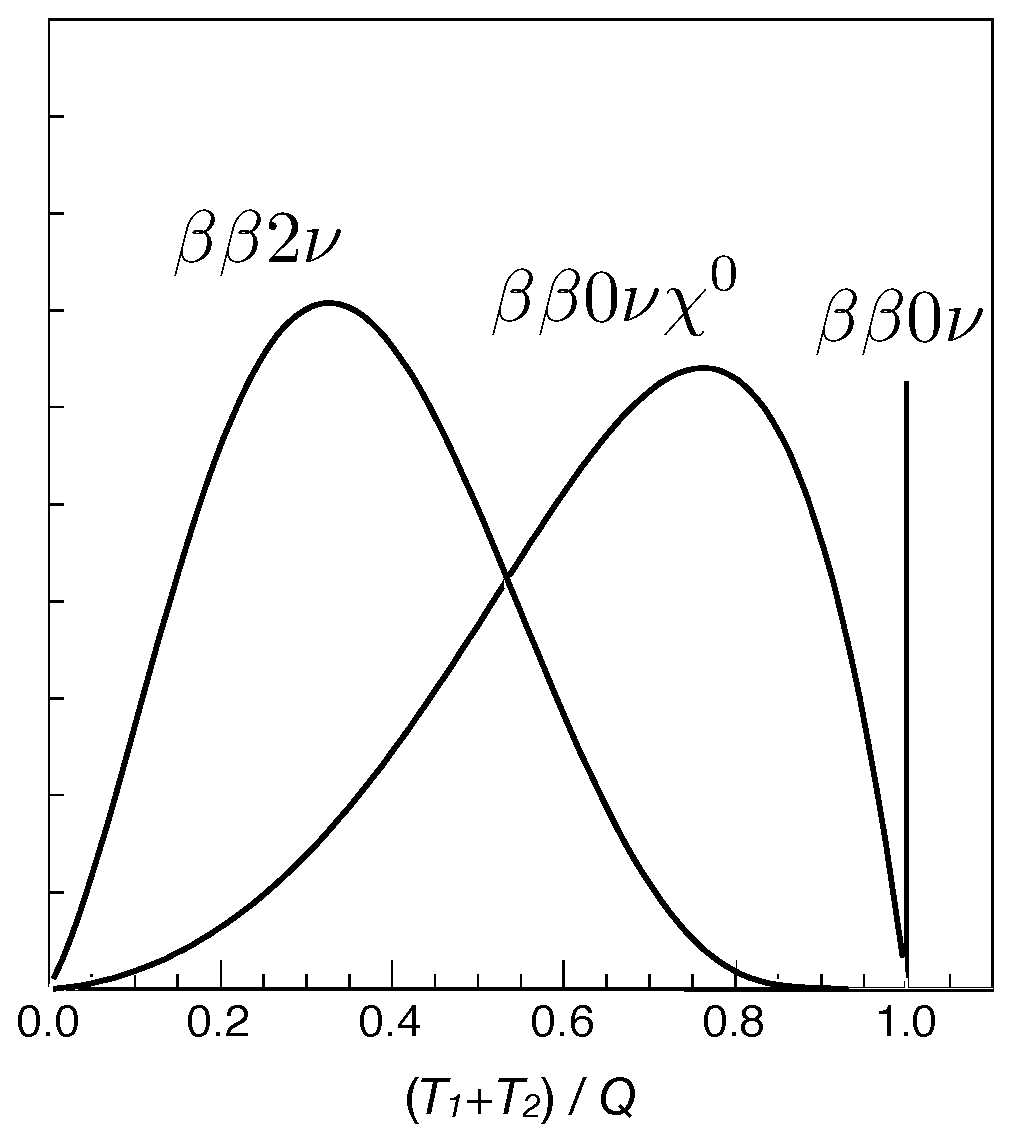
\includegraphics[angle=0,scale=0.325]{img/modes.eps}
\end{center}
\caption{Spectra for the sum kinetic energy $T_1+T_2$ of the two electrons, for different \bb\ modes: \bbtnu, \bbonu, and \bb\ decay with Majoron emission.} \label{fig:modes}
\end{figure}

While in the following we will focus on \bbonu\ as defined in Eq.~(\ref{eq:bb0nu}), there are three closely related lepton number violating processes that can be investigated:
%
\begin{eqnarray}
\beta^+\beta^+0\nu: & (Z,A) \to (Z-2,A) + 2\ e^+  \label{eq:b+b+}\\
\beta^+\text{EC}0\nu: & e^- + (Z,A) \to (Z-2,A) + e^+ \label{eq:b+EC}\\
\text{ECEC}0\nu: & 2\ e^- + (Z,A) \to (Z-2,A)^\ast \label{eq:ECEC}
\end{eqnarray}
%
Such processes are called \emph{double positron emission}, \emph{single positron emission plus single electron capture} (EC), and \emph{double electron capture}, respectively. All three involve transitions where the nuclear charge decreases (as opposed to increasing, as in \bbonu) by two units. From the the theoretical point of view, the physics probed by $\beta^+\beta^+0\nu$, $\beta^+\text{EC}0\nu$ and $\text{ECEC}0\nu$ is identical to the one probed by \bbonu. From the experimental point of view, however, $\beta^+\beta^+0\nu$ and $\beta^+\text{EC}0\nu$ are less favorable than \bbonu\ because of the smaller phase space available. On the other hand, the process $\text{ECEC}0\nu$ is gaining some attention recently as a promising (but still much less developed) alternative to \bbonu, since a resonant enhancement of its rate can in principle occur \cite{Eliseev:2011zza}.

In the following, the neutrinoless mode \bbonu\ is discussed in more detail, from both the theoretical and experimental point of views.

\subsection{The black box theorem } \label{subsec:bb0nu_blackbox}
In general, in theories beyond the Standard Model there may be several sources of total lepton number violation which can lead to \bbonu. Nevertheless, as it was first pointed out in reference \cite{Schechter:1981bd}, irrespective of the mechanism, \bbonu\ necessarily implies Majorana neutrinos. This is called the \emph{black box} (or Schechter-Valle) theorem. The reason is that any $\Delta L\neq 0$ diagram contributing to the decay would also contribute to the $(e,e)$ entry of the Majorana neutrino mass matrix, $(m_{\nu})_{ee}$. This is shown in fig.~\ref{fig:blackbox}, where a $\bar{\nu}_e-\nu_e$ transition, that is a non-zero $(m_{\nu})_{ee}$, is induced as a consequence of any $\Delta L\neq 0$ operator responsible for \bbonu.

From a quantitative point of view, however, the diagram in fig.~\ref{fig:blackbox} corresponds to a tiny (of order $\mathcal{O}(10^{-28}~\mathrm{eV})$) mass generated at the four-loop level, and is far too small to explain the neutrino mass splittings observed in neutrino oscillation experiments \cite{Duerr:2011zd}. Other, unknown, Majorana and/or Dirac mass contributions must exist. As a consequence, therefore, the black box theorem says nothing about the physics mechanism dominating a \bbonu\ rate that is large enough to be observable. The dominant mechanism leading to \bbonu\ could then either be directly connected to neutrino oscillations phenomenology, or only indirectly connected or not connected at all to it \cite{Rodejohann:2011mu}. The former case is realized in the standard \bbonu\ mechanism of light neutrino exchange, discussed in Sect.~\ref{subsec:bb0nu_lightmajoranaexchange}. The latter case involves alternative \bbonu\ mechanisms, briefly outlined in Sect.~\ref{subsec:bb0nu_alternativemechanisms}.

\begin{figure}[t!b!]
\begin{center}
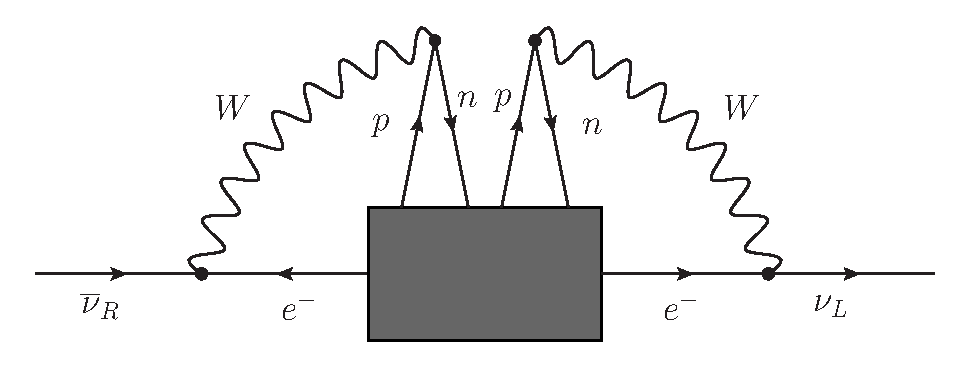
\includegraphics[scale=0.65]{img/blackbox.eps}
\end{center}
\caption{Diagram showing how any neutrinoless double beta decay process induces a $\bar{\nu}$-to-$\nu$ transition, that is, an effective Majorana mass term. This is the so-called \emph{black box theorem} \cite{Schechter:1981bd}.} \label{fig:blackbox}
\end{figure}


\subsection{The standard neutrinoless double beta decay mechanism: light Majorana neutrino exchange} \label{subsec:bb0nu_lightmajoranaexchange}

Neutrinoless double beta decay can arise from a diagram (fig.~\ref{fig:bb0nu_standardmechanism}) in which the parent nucleus emits a pair of virtual $W$ bosons, and then these $W$ exchange a Majorana neutrino to produce the outgoing electrons. The rate is non-zero only for massive, Majorana neutrinos. The reason is that the exchanged neutrino in fig.~\ref{fig:bb0nu_standardmechanism} can be seen as emitted (in association with an electron) with almost total positive helicity. Only its small, $\mathcal{O}(m/E)$, negative helicity component is absorbed in the other vertex by the Standard Model electroweak current. Considering that the amplitude is in this case a sum over the contributions of the three light neutrino mass states $\nu_i$, and that is also proportional to $U_{ei}^2$, we conclude that the modulus of the amplitude for the \bbonu\ process must be proportional in this case to the \emph{effective neutrino Majorana mass}:
%
\begin{equation}
\mbb \equiv \lvert \sum_{i=1}^{3} m_i U_{ei}^2 \rvert. \label{eq:mbb}
\end{equation}
%
In other words, the effective neutrino Majorana mass corresponds to the modulus of the $(e,e)$ element of the neutrino mass matrix of eq.~(\ref{eq:mnu}), $\mbb\equiv \lvert (m_{\nu})_{ee}\rvert$.

%%%%%
\begin{figure}[t!b!]
\begin{center}
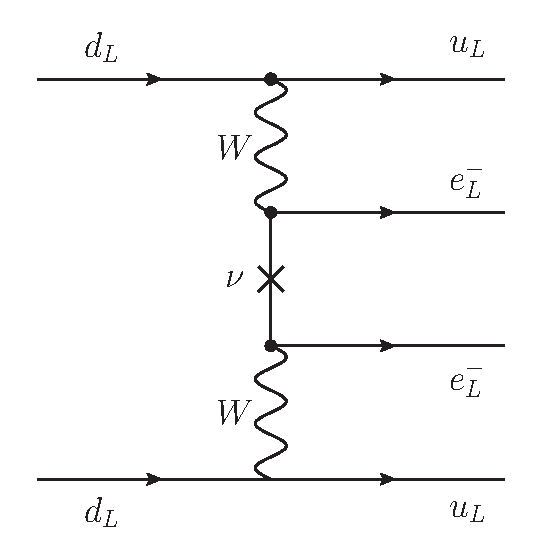
\includegraphics[scale=0.55]{img/FD_lightnu.eps}
\end{center}
\caption{\label{fig:bb0nu_standardmechanism}The standard mechanism for \bbonu\ decay, based on light Majorana neutrino exchange.}   
\end{figure}
%%%%%

In the case where light Majorana neutrino exchange is the dominant contribution to \bbonu, the inverse of the half-life for the process can be written as \cite{Doi:1985dx}:
%
\begin{equation}
\frac{1}{T^{0\nu}_{1/2}} = G^{0\nu}(Q,Z)\ \lvert M^{0\nu}\rvert^2\ \mbb^2,
\label{eq:Tonu}
\end{equation}
%
where \Gonu\ is a phase space factor that depends on the transition $Q$-value and on the nuclear charge $Z$, and $M^{0\nu}$ is the nuclear matrix element (NME). The phase space factor can be calculated analytically, in principle, with reasonable accuracy\footnote{An accurate description of the effect of the nuclear Coulomb field on the decay electron wave-functions is, however, required.}. The  NME is evaluated using nuclear models, although with considerable uncertainty (see Sect.~\ref{sec:nme}).
In other words, the value of the effective neutrino Majorana mass \mbb\ in eq.~(\ref{eq:mbb}) can be inferred from a non-zero \bbonu\ rate measurement, albeit with some nuclear physics uncertainties. Conversely, if a given experiment does not observe the \bbonu\ process, the result can be interpreted in terms of an upper bound on \mbb.  

If light Majorana neutrino exchange is the dominant mechanism for \bbonu, it is clear from eq.~(\ref{eq:mbb}) that \bbonu\ is in this case directly connected to neutrino oscillations phenomenology, and that it also provides direct information on the absolute neutrino mass scale, as cosmology and $\beta$ decay experiments do (see Sect.~\ref{subsec:massivenus_whereweare}). The relationship between \mbb\ and the actual neutrino masses $m_i$ is affected by:
%
\begin{enumerate}
\item the uncertainties in the measured oscillation parameters;
\item the unknown neutrino mass ordering (normal or inverted);
\item the unknown phases in the neutrino mixing matrix (both Dirac and Majorana). 
\end{enumerate}
%

For example, the relationship between \mbb\ and the lightest neutrino mass $m_{\text{light}}$ (which is equal to $m_1$ or $m_3$ in the normal and inverted mass ordering cases, respectively) is illustrated in fig.~\ref{fig:mbetabetavsmlight}. This graphical representation was first proposed in \cite{Vissani:1999tu}. The width of the two bands is due to items 1 and 3 above, where the uncertainties in the measured oscillation parameters (item 1) are taken as $3\sigma$ ranges from a recent global oscillation fit \cite{Esteban:2020cvm}. Figure \ref{fig:mbetabetavsmlight} also shows a 90\% confidence level upper bound on \mbb\ from current \bbonu\ data ($m_{\beta\beta}<0.036-0.156\ \text{eV}$), which we will discuss in Sect.~\ref{subsec:bb0nu_expstatus}. As can be seen from fig.~\ref{fig:mbetabetavsmlight}, current \bbonu\ data provide a constraint on the absolute mass scale $m_{\text{light}}$ that is more competitive than the current one from $\beta$ decay decay experiments, although less competitive as the cosmological one.
%
\begin{figure}[t!b!]
\begin{center}
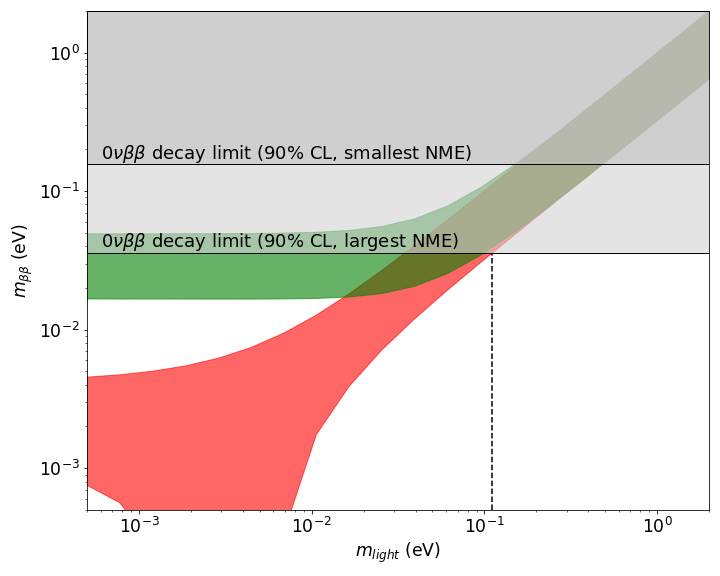
\includegraphics[width=0.7\textwidth]{img/mbetabetavsmlight.png}
\end{center}
\caption{\label{fig:mbetabetavsmlight}The effective neutrino Majorana mass \mbb\ as a function of the lightest neutrino mass, $m_{\text{light}}$. The red (green) band corresponds to the normal (inverted) ordering, respectively, in which case $m_{\text{light}}$ is equal to $m_1$ ($m_3$). The horizontally-excluded region comes from \bbonu\ constraints.}
\end{figure}

In figs.~\ref{fig:mass_constraints_cosmo_beta} and \ref{fig:mbetabetavsmlight}, we have shown only upper bounds on various neutrino mass combinations, coming from current data. The detection of positive results for absolute neutrino mass scale observables would open up the possibility to further explore neutrino properties and lepton number violating processes. We give three examples in the following. First, the successful determination of both $m_{\beta}$ in eq.~(\ref{eq:mbeta}) and \mbb\ in eq.~(\ref{eq:mbb}) via $\beta$ and \bbonu\ decay experiments, respectively, can in principle be used to determine or constrain the phases $\alpha_{i}$ \cite{Avignone:2007fu}. Second, measurements of $m_{\beta}$ or $m_{\text{cosmo}}$ in eq.~(\ref{eq:mcosmo}) may yield a constraint on $m_{\text{light}}$ that is inconsistent with a \mbb\ upper limit. In this case, the non-observation of \bbonu\ would suggest that neutrinos are Dirac particles. Third, measurements of $m_{\beta}$ or $m_{\text{cosmo}}$ may yield a constraint on $m_{\text{light}}$ that is inconsistent with a measured non-zero \mbb. This scenario would demonstrate that additional lepton number violating physics, other than light Majorana neutrino exchange, is at play in the \bbonu\ process. We briefly describe some of these possible \bbonu\ alternative mechanisms in the following.


\subsection{Alternative neutrinoless double beta decay mechanisms} \label{subsec:bb0nu_alternativemechanisms}
A number of alternative \bbonu\ mechanisms have been proposed. For an excellent and complete discussion of those, we refer the reader to \cite{Rodejohann:2011mu}. The realization of \bbonu\ can differ from the standard mechanism in one or several aspects:
%
\begin{itemize}
\item The Lorentz structure of the currents. Positive chirality currents mediated by a $W_R$ boson can arise, for example, in left-right symmetric theories. A possible diagram involving positive chirality current interactions of heavy Majorana neutrinos $N_i$ is shown in fig.~\ref{fig:nonstandardmechanisms}(a).
%
\item The mass scale of the exchanged virtual particles. One example would be the presence of ``sterile'' (that is, described by positive chirality fields) neutrinos, either light or heavy, in the neutrino propagator of fig.~\ref{fig:bb0nu_standardmechanism}, in addition to the three light, active, neutrinos we are familiar with. Another example would be the exchange of heavy supersymmetric particles, as in fig.~\ref{fig:nonstandardmechanisms}(b).
%
\item The number of particles in the final state. A popular example involves decay modes where additional Majorons, that is very light or massless particles which can couple to neutrinos, are produced in association with the two electrons (see fig.~\ref{fig:nonstandardmechanisms}(c)).
\end{itemize}
%
\begin{figure}[t!b!]
\begin{center}
\begin{tabular}{ccc}
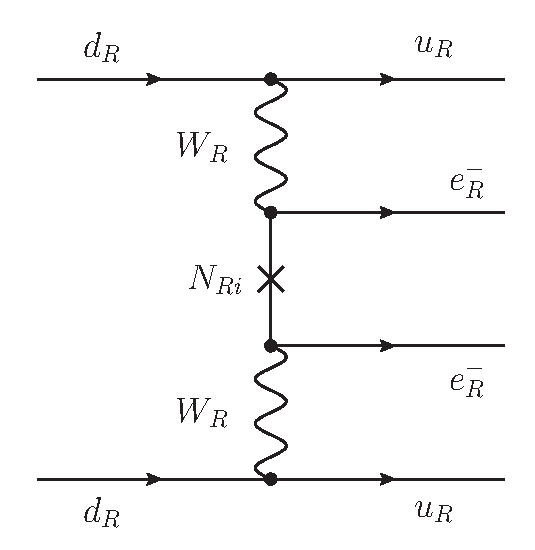
\includegraphics[width=0.30\textwidth]{img/FD_heavyNR_LR.eps} &
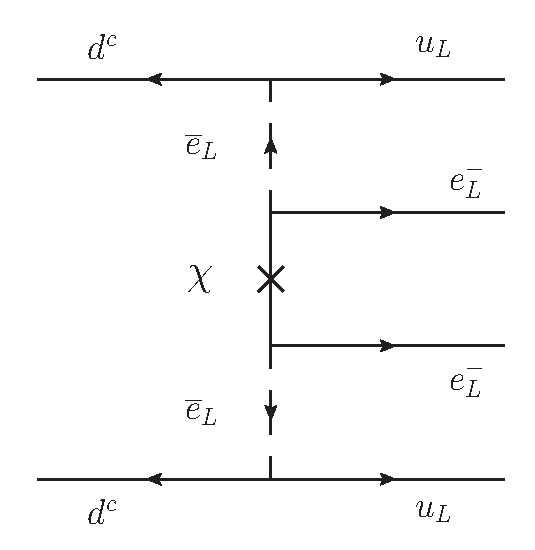
\includegraphics[width=0.30\textwidth]{img/FD_RPV_1a.eps} &
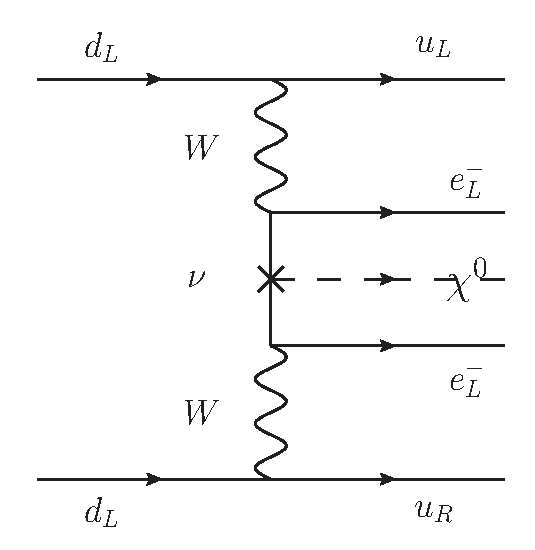
\includegraphics[width=0.30\textwidth]{img/FD_Majoron.eps} \\
(a) & (b) & (c) \\
\end{tabular}
\end{center}
\caption{\label{fig:nonstandardmechanisms}Examples of non-standard mechanism for \bbonu: (a) heavy neutrino exchange with positive chirality currents \cite{Mohapatra:1986pj}; (b) neutralino exchange in R-parity violating supersymmetry \cite{Mohapatra:1986su}; (c) Majoron emission \cite{Georgi:1981pg}.}   
\end{figure}
%
In non-standard \bbonu\ mechanisms, the scale of the lepton number violating physics is often larger than the characteristic nuclear Fermi momentum scale $\mathcal{O}$(100~MeV), in which case one speaks of \emph{short-range} processes. This is the case when the \bbonu\ process is mediated by heavy particles. It is in contrast to the standard \bbonu\ mechanism of light Majorana neutrino exchange, in which case the neutrino is very light compared to this momentum transfer scale, resulting in a \emph{long-range} process. Non-standard and long-range \bbonu\ processes are, however, also possible.

In general, several contributions to the total \bbonu\ amplitude can add coherently, allowing for interference effects. Neutrinoless double beta decay observables alone may be able to identify the dominant mechanism responsible for \bbonu. We give three examples. First, if Majorons are also emitted in association with the two electrons, energy conservation alone requires the electron kinetic energy sum $T_1+T_2$ to be a continuous spectrum with $Q_{\beta\beta}$ as endpoint. This spectrum is potentially distinguishable from the \bbtnu\ one (see fig.~\ref{fig:modes}), provided that the Majoron-neutrino coupling constant is large enough. Second, if positive chirality current contributions dominate the \bbonu\ rate, electrons will be emitted predominantly as positive helicity states. As a consequence, both the energy and angular correlation of the two emitted electrons will be different from the ones of the standard \bbonu\ mechanism. A detector capable of reconstructing individual electron tracks may therefore be able to distinguish this type of non-standard \bbonu\ mechanism from light Majorana neutrino exchange (see, for example, \cite{SuperNEMO:2010wnd}). Third, the combined observation of \bbonu\ decays to both ground and excited states of the daughter isotope may also shed light on the \bbonu\ mechanism. Neutrinoless double beta decays to excited states are however harder to search for, given the lower reaction Q-values and hence lower predicted rates. On the other hand, their experimental signature would be very characteristic, with typically one or two gamma rays emitted in coincidence with the two decay electrons. 
%

%\subsection{Existing experimental results} \label{subsec:bb0nu_expstatus}
%Neutrinoless double beta decay searches have been carried out over more than half a century, exploiting the same experimental techniques used for measuring the two-neutrino mode rate. Several \bb\ emitting isotopes have been investigated, as shown in table \ref{tab:bb0nu_exp}. Table~\ref{tab:bb0nu_exp} shows the best current \bbonu\ limits for the same 9 isotopes for which direct \bbtnu\ decay direct measurements exist, and includes also a recent limit for \Te{128}  (for which a direct measurement of the two-neutrino mode remains elusive).
%
%\begin{table}[t!b!]
%\centering
%\caption{\label{tab:bb0nu_exp}Current best limits on the half-life of \bbonu\ processes for the most interesting isotopes. All values are at 90\% CL.}
%\begin{tabular}{rcl}
%\toprule
%Isotope & $T_{1/2}^{0\nu}\ \text{(years)}$ & Experiment \\ \midrule
%%
%\Ca{48} & $>5.8 \times 10^{22}$ & ELEGANT VI \cite{Umehara:2008ru} \\
%%
%\Ge{76} & $>1.8 \times 10^{26}$ & GERDA \cite{GERDA:2020xhi} \\
%%
%\Se{82} & $>4.6 \times 10^{24}$ & CUPID-0 \cite{CUPID:2022puj} \\
%%
%\Zr{96} & $>9.2 \times 10^{21}$ & NEMO-3 \cite{NEMO-3:2009fxe}  \\
%%
%\Mo{100} & $>1.8 \times 10^{24}$ & CUPID-Mo \cite{Augier:2022znx}  \\
%%
%\Cd{116} & $>2.2 \times 10^{23}$ & Aurora \cite{Barabash:2018yjq}   \\
%%
%\Te{128} & $>3.6 \times 10^{24}$ & CUORE \cite{CUORE:2022piu} \\
%%
%\Te{130} & $>2.2 \times 10^{25}$ & CUORE \cite{CUORE:2021mvw} \\
%%
%\Xe{136} & $>2.3 \times 10^{26}$ & KamLAND-Zen \cite{KamLAND-Zen:2022tow} \\
%%
%\Nd{150} & $>2.0 \times 10^{22}$ & NEMO-3 \cite{NEMO-3:2016qxo} \\
%\bottomrule
%%\end{narrowtabular}
%\end{tabular}
%\end{table}
%%%%%%
%
%The most sensitive half-life limit to date was set by the xenon-based KamLAND-Zen experiment \cite{KamLAND-Zen:2022tow}: $\Tonu(\Xe{136}) > 2.3 \times 10^{26}$ years (90\% CL), corresponding to an effective Majorana mass bound of $\mbb < 0.036-0.151$~eV, where the range covers  commonly adopted nuclear matrix element calculations. Particularly competitive limits also exist for \Ge{76} and \Te{130}. For \Ge{76}, the GERDA experiment reported final half-life and Majorana mass limits of $\Tonu(\Ge{76})>1.8\times 10^{26}$~yr and $\mbb<0.079-0.180$~eV at 90\% CL, respectively \cite{GERDA:2020xhi}. For \Te{130}, the latest limits from the CUORE experiment are $\Tonu(\Te{130})>2.2\times 10^{25}$~yr and $\mbb<0.090-0.305$~eV at 90\% CL, respectively \cite{CUORE:2021mvw}. It is worth noting that, despite its lower half-life reach, the CUORE result is almost as competitive as the KamLAND-Zen and GERDA ones in terms of Majorana mass reach. As we will see in Sections \ref{sec:nme} and \ref{sec:ingredients}, this is due to the favorable phase space factor and nuclear matrix element of \Te{130}, compared to \Xe{136} and \Ge{76}.   
%






